\documentclass[sigconf]{acmart}

\usepackage[english]{babel}
\usepackage{blindtext}
\usepackage{indentfirst}

% Copyright
\renewcommand\footnotetextcopyrightpermission[1]{} % removes footnote with conference info
\setcopyright{none}
%\setcopyright{acmcopyright}
%\setcopyright{acmlicensed}
%\setcopyright{rightsretained}
%\setcopyright{usgov}
%\setcopyright{usgovmixed}
%\setcopyright{cagov}
%\setcopyright{cagovmixed}

\settopmatter{printacmref=false, printccs=false, printfolios=true}

% DOI
\acmDOI{}

% ISBN
\acmISBN{}

%Conference
%\acmConference[Submitted for review to SIGCOMM]{}
%\acmYear{2018}
%\copyrightyear{}

%% {} with no args suppresses printing of the price
\acmPrice{}


\begin{document}
\title{Network-Ordered Paxos on a Cloud Platform}

%\titlenote{Produces the permission block, and copyright information}
%\subtitle{Extended Abstract}

\author{Emma Dauterman, Zo{\"e} Bohn}
% \author{Firstname Lastname}
% \authornote{Note}
% \orcid{1234-5678-9012}
% \affiliation{%
%   \institution{Affiliation}
%   \streetaddress{Address}
%   \city{City} 
%   \state{State} 
%   \postcode{Zipcode}
% }
% \email{email@domain.com}

% The default list of authors is too long for headers}
\renewcommand{\shortauthors}{Dauterman, Bohn}

\begin{abstract}
We present our evaluation of Network-Ordered Paxos \cite{nopaxos} (NOPaxos) by Li et. al. on a cloud platform. We describe the motivation for the NOPaxos protocol and discuss the extensions to the original software required when running on a cloud platform. We then compare the throughput/latency and scaling capacities of NOPaxos on a cloud platform to those of NOPaxos on dedicated hardware by reproducing Figures 5 and 8 from the original paper \cite{nopaxos}. 
\end{abstract}

\maketitle

\section{Introduction}

\indent Today's data center applications depend on replication to ensure data availability and transparently mask server failures. Unfortunately, consensus protocols like Paxos\cite{paxos,paxossimple} and Raft\cite{raft} that provide replication with strong consistency guarantees also impose a significant performance overhead. Network-Ordered Paxos\cite{nopaxos} (NOPaxos) dramatically reduces this performance overhead by splitting the replication responsibility between the network and protocol layers. The authors of NOPaxos present a new network primitive to do this: ordered unreliable multicast (OUM). 

OUM provides semantics strong enough to reduce overhead at the protocol layer, but weak enough that OUM can be implemented at near-zero-cost within a datacenter. OUM is asynchronous and unreliable, and it guarantees that all replicas receive messages in the same order. All packets for a OUM group are routed through a single sequencer, which determines the global packet order. The authors describe three places in the network to implement the sequencer: in the switches themselves, in hardware middleboxes, and at end-hosts. OUM greatly simplifies the task of the protocol layer: instead of agreeing on the total ordering of client requests, now replicas only have to agree on which requests to execute and which to permanently ignore. 

\subsection{NOPaxos on a Cloud Platform}
    
Cloud platforms have become increasingly popular because they allow users to pay for resources used without significant up-front investment and they move the burden of maintaining a cluster from the user to the cloud provider. Unfortunately, NOPaxos as presented in the original paper \cite{nopaxos} cannot run on a cloud platform because it relies on multicast. Most mainstream cloud providers such as Amazon AWS and Google Cloud Platform do not support multicast because all instances run on the same internal network, and so multicast could overload the network and negatively impact performance. 

Given the advantages of cloud platforms, we explore adapting NOPaxos to a cloud platform and evaluate its performance in this environment with the necessary modifications. Specifically, we compare the throughput, latency, and scaling capabilities of NOPaxos to those of three other consensus protocols (paxos, paxos with batching, and fastpaxos) and an unreplicated system when running on a cloud platform. We contrast these results with those of the original NOPaxos paper \cite{nopaxos}, which conducted its evaluation on dedicated hardware.

We find that the modifications necessary to allow NOPaxos to run on a cloud platform create a bottleneck that prevent it from scaling as it does on dedicated hardware. Therefore, although NOPaxos on a cloud platform can achieve comparable latency under low load, it is unable match the throughput achieved on dedicated hardware with a greater number of replicas. However, we show that in some circumstances, NOPaxos in the cloud still performs better than other consensus protocols in the same environment.

The reminder of the paper proceeds as follows. In Section 2, we discuss related work regarding the reduction of replication overhead in consensus protocols and how this compares to NOPaxos, especially in the context of testing on cloud platforms. In Section 3, we outline the design and setup of our experiments with NOPaxos on a cloud platform, including the modifications that had to be made to the original code base. In Section 4, we contrast the results of these experiments with those run by the authors of \cite{nopaxos} on dedicated hardware, focusing in particular on our reproductions of Figures 5 and 8 from the original paper; we also identify and evaluate the bottleneck that we discovered during the course of these experiments. In Section 5, we discuss the limitations of our experiment and of NOPaxos on a cloud platform. In Section 6, we outline future work for the development and evaluation of consensus protocols (such as NOPaxos) on cloud platforms. Finally, in Section 6, we conclude with a summary of our results and lessons learned. 
\section{Related Work} \label{related}

Other consensus protocols have also tried to reduce the performance overhead of replication. \cite{pbft} shows how vanilla Paxos can be modified to batch requests, using a sliding-window where the system adaptively adjusts the batch size. This is shown to reduce latency at low load while still providing throughput benefits at high load \cite{pbft}.

Speculative Paxos\cite{specpaxos} and NetPaxos\cite{netpaxos} take a similar approach to NOPaxos by pushing functionality into the network (and thus also require modifications to run on a cloud platform).

Speculative Paxos uses a Mostly-Ordered Multicast primitive that provides a best-effort ordering property, but because it is not a guarantee, both superquorums and speculation are necessary. NOPaxos avoids protocol complexity by pushing more responsibility into the network layer. Conversely, NetPaxos moves Paxos logic into the switches (using P4), requiring switches to store the results of each consensus instance, which could become a large amount of state. While NetPaxos requires changes to the switch firmware, NOPaxos has much more realistic expectations of switches, requiring only the OUM primitive. For these reasons, we chose to modify and evaluate NOPaxos over SpecPaxos and NetPaxos. 

Fast Paxos\cite{fastpaxos}, Generalized Paxos\cite{generalizedpaxos}, and Egalitarian Paxos\cite{epaxos} (EPaxos) take a different approach, making no assumptions about the network (and thus do not require modifications to run on a cloud platform). 

Fast Paxos allows clients to send operations directly to replicas to reduce overhead, but if multiple clients concurrently send operations, competing to commit, extra messages are required to determine ordering (NOPaxos relies on the network to do this). Generalized Paxos and EPaxos both exploit commutativity to improve performance: Generalized Paxos is similar to Fast Paxos but solves the problem of contention with multiple cilents by exploiting commutativity, and EPaxos uses multiple leaders to propose and execute operations concurrently. For both Generalized Paxos and EPaxos, performance depends on the nature of the workload (i.e. the degree of commutativity), and so cannot achieve the consistency of performance across workloads in NOPaxos. However, these protocols make no assumptions about the network, and so are good choices outside datacenters. 

The authors of the original paper\cite{nopaxos} compare NOPaxos to both Speculative Paxos and Fast Paxos (in addition to vanilla Paxos and Paxos with Batching) on dedicated hardware. We likewise include a comparison of NOPaxos to Fast Paxos, vanilla Paxos, and Paxos with Batching on a cloud platform. However, due to time constraints and the need for modifications to the original protocol, we leave a comparison of NOPaxos to Speculative Paxos on a cloud platform to future work. 
\section{Experiment Design}

To run our experiments, we extended the NOPaxos code base created by the authors of \cite{nopaxos}: 
\par \quad \textit{https://github.com/UWSysLab/NOPaxos}.
\newline
Our fork of this code base is available at: 
\par \quad \textit{https://github.com/edauterman/NOPaxos}. 
\newline
\par We leveraged the existing benchmarking code to compare NOPaxos to four other protocols: Fast Paxos, Paxos, Paxos with Batching, and (as a baseline) an unreplicated protocol. As stated previously, we did not evaluate Speculative Paxos (as the original paper does) due to time and cloud platform constraints. 

To minimize microsecond-level latency, we removed existing print statements from the benchmarking code, which we found noticeably improved throughput and latency. 

For consistency with the original dedicated hardware experiments, we collect our throughput/latency measurements with five active replica nodes. In addition, all latency measurements are of average latency, and all Paxos with Batching measurement were taken with a maximum batch size set to 64 (although this information is not included in the original paper \cite{nopaxos}, we were able to communicate with the authors directly about these parameters).

For all experiments, we run five dedicated client machines and add more concurrent client threads to increase throughput as necessary, as suggested by the authors of \cite{nopaxos}. Each client thread simultaneously makes 1,000 requests. In addition, each data point reported in our evaluation is the average of 10 runs of the experiment with identical parameters, necessary to reduce variation between runs when measuring microsecond-level latencies. We found that averaging across at least 5 runs was critical for reproducability, but we saw diminishing returns using between 5 and 10 runs. 


\subsection{Cloud Platform}

We ran all of our experiments on the Google Cloud (gcloud) platform. We used a total of 15 compute nodes (9 replicas, 5 clients, and 1 sequencer). All nodes are located in the same geographic zone (us-west1-a); we found that placing nodes in different zones negatively impacted performance by several orders of magnitude; thus a system that is geo-replicated should not expect to be able to reproduce the results we show in this paper. 

The replica compute nodes and the sequencer have IP forwarding enabled so that the sequencer can properly forward packets to the replicas; we also experimented with packet encapsulation, which allowed us to run NOPaxos without IP forwarding enabled. However, we found that this had a (small) negative impact on performance due to additional overhead.

\subsection{Sequencer Modifications}

Recall that in NOPaxos, all packets for a OUM group are routed through a single sequencer, determining the global packet order. The sequencer can be implemented in one of three locations in the network: in the switches themselves, in hardware middleboxes, and at end-hosts. At the time of the paper, programmable switches that could implement OUM were not commercially available and so the authors performed most of their evaluation using a hardware middlebox sequencer. Because cloud platforms preclude the programming of switches or the insertion of middleboxes, we chose to use implement the sequencer at the end-host. This required creating a sequencer node to route all packets through. 

The NOPaxos code base includes the implementation in C++ for the sequencer using a raw socket. However, because most cloud platforms do not support multicast, we had to adapt the sequencer to run without multicast. Per the suggestion of the authors, we modified the end-host sequencer to send individual copies of packets to each replica in place of multicast. To preserve the original client source address, the end-host sequencer simply forwards client packets to replicas.

\subsection{Reproducibility}

We extended the NOPaxos code base with a script to automate the collection of all measurements taken for our evaluation, including figure generation. For details, see the README at \textit{https://github.com/edauterman/NOPaxos}.  

\section{Evaluation}

We address the following questions in our evaluation:
\begin{enumerate}
\item How does NOPaxos's performance on a cloud platform compare to its performance on dedicated hardware?
\item How do the modifications to NOPaxos required for a cloud platform affect its ability to scale?
\end{enumerate}

\begin{figure}[tp]
\centering
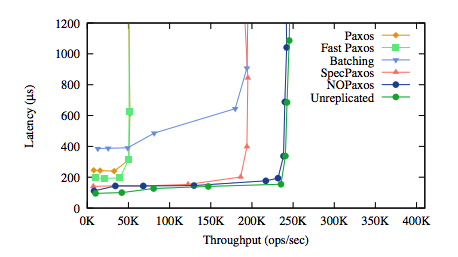
\includegraphics[scale=0.5]{figures/figure_5.png}
\caption{Original Figure 5 in \cite{nopaxos}, showing latency vs. throughput comparison for NOPaxos and other protocols}
\end{figure}

\begin{figure}[tp]
\centering
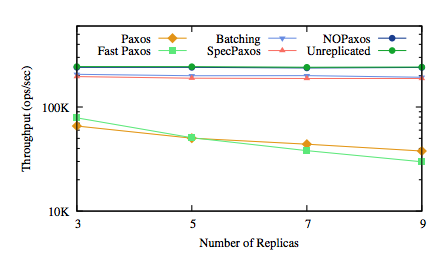
\includegraphics[scale=0.5]{figures/figure_8.png}
\caption{Original Figure 8 in \cite{nopaxos}, showing maximum throughput with increasing number of replicas}
\end{figure}

\subsection{NOPaxos: Dedicated Hardware}

\cite{nopaxos} shows that on dedicated hardware using a hardware middlebox sequencer, NOPaxos on achieves a throughput within 2\% and latency within 16 microseconds of an unreplicated system, better than any existing consensus protocol. NOPaxos continues to maintain a throughput comparable to an unreplicated system as the number of replicas increases. The throughput and latency results are presented in Figure 5 of \cite{nopaxos} and the scaling results in Figure 8, both included here for reference (Figures 1 and 2). Note that because we use the end-host sequencer implementation, our NOPaxos results are more directly comparable to Figure 6 of \cite{nopaxos}; however, Figure 6 shows that the performance of NOPaxos with an end-host sequencer is very similar to that of NOPaxos with a hardware middlebox sequencer, with comparable throughput and only a slight increase in latency; therefore we include Figure 5, as it shows the performance of NOPaxos in relation to the other evaluated consensus protocols. 

\subsection{NOPaxos: Cloud Platform}

\begin{figure}[tp]
\centering
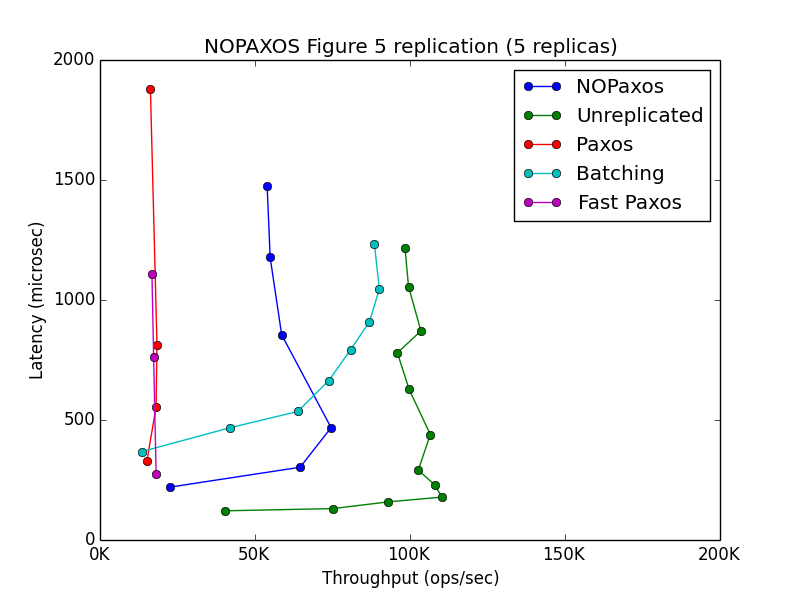
\includegraphics[scale=0.5]{figures/Figure5-5.png}
\caption{Reproduction of Figure 5 in \cite{nopaxos} with 5 replicas, showing latency vs. throughput comparison for NOPaxos and other protocols}
\end{figure}

\begin{figure}[tp]
\centering
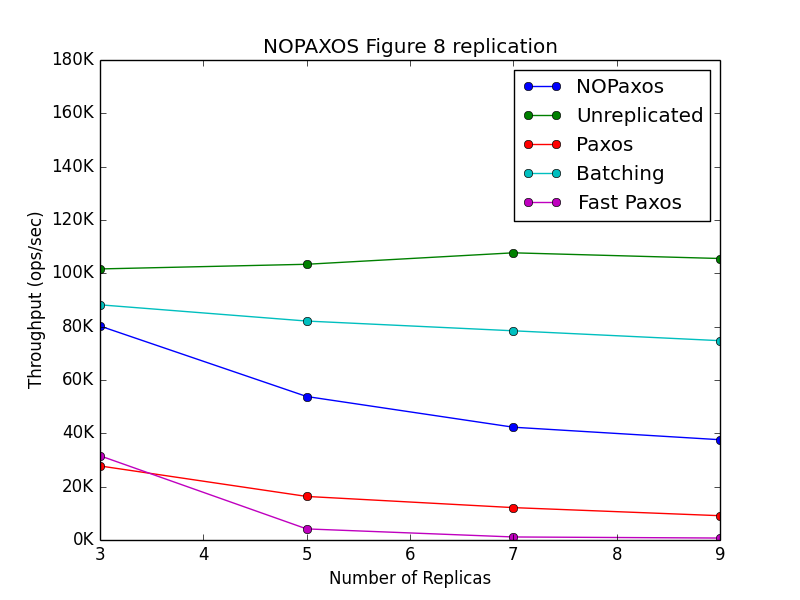
\includegraphics[scale=0.5]{figures/Figure8.png}
\caption{Reproduction of Figure 8 in \cite{nopaxos}, showing maximum throughput with increasing number of replicas}
\end{figure}

\textbf{Throughput/Latency: }We present the throughput and latency results of our experiments in Figure 3, preserving the formatting of the original paper's Figure 5 for comparison. We can see that the relative performances of Paxos, Fast Paxos, Batching (Paxos with Batching), and Unreplicated on the cloud platform reflect the results of the dedicated hardware experiments performed by the authors. Paxos and Fast Paxos both have very low maximum throughput, although Fast Paxos has slightly lower latency, and Batching gets closer to the throughput of Unreplicated, although with much higher latency.

NOPaxos, however, has a noticeable difference in its performance relative to the other consensus protocols when run on a cloud platform rather than dedicated hardware. Although it continues to achieve considerably lower latency than the other (replicated) protocols prior to reaching its maximum throughput, this maximum throughput is significantly lower (in comparison to the other protocols) on a cloud platform than on dedicated hardware. Thus we conclude that the modifications to the protocol required for a cloud platform have introduced (or exacerbated) a bottleneck in the protocol (further discussion in \ref{bottleneck}). 

\textbf{Scalability: }Again, for comparison, we present the scalability results of our experiments in Figure 4 with the same format as Figure 8 of the original paper. As with the previous figure, we see similar relative performances of Paxos, Fast Paxos, Batching, and Unreplicated on a cloud platform as with dedicated hardware: Unreplicated achieves the highest throughput with Batching achieving just slightly lower throughput, and this throughput does not drop with an increasing number of replicas for either protocol; Fast Paxos does not scale as well as Paxos as the number of replicas increases.

However, we again see a difference in performance for NOPaxos. In the original dedicated hardware experiments, NOPaxos had performance nearly identical to Unreplicated; on a cloud platform, NOPaxos is outperformed by both Unreplicated and Batching as the number of replicas increases, and its throughput drops. These results again suggest the presence of a bottleneck introduced or exacerbated by our modifications (further discussion in \ref{bottleneck}). We additionally conclude from this data that in a cloud platform environment, NOPaxos is best used in situations requiring only a small number of replicas. 

For both figures, the maximum throughput we observed is approximately a factor of two lower than the throughput reported by the authors. We expected such a difference to occur when migrating from dedicated hardware to a multi-tenant datacenter environment where link capacity is shared between many tenants. Our graphs also indicate more variation (the lines are less "smooth"), again most likely due to the different testing environments.

\textbf{NOPaxos with Fewer Replicas: }As stated previously in our analysis of Figure 4 (our Figure 8 reproduction), it is clear that NOPaxos on a cloud platform performs better with fewer replicas. We therefore chose to evaluate the latency and throughput of NOPaxos on the cloud with only 3 replicas (fewer than used in the original NOPaxos paper) to see if we could achieve results closer to those on dedicated hardware; while more replicas are desirable to achieve greater fault-tolerance, 3 replicas are sufficient for replication and a fault-tolerance factor of 1, which may be sufficient for some systems. 

\begin{figure}[tp]
\centering
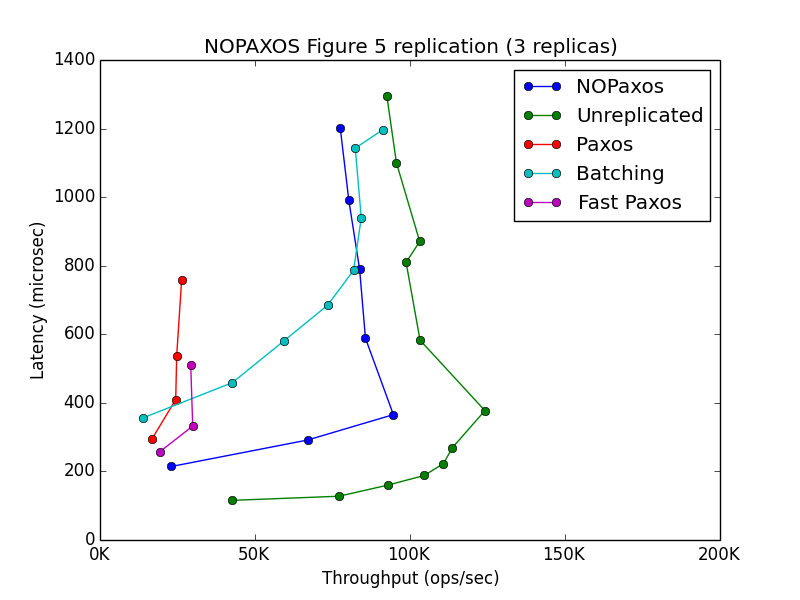
\includegraphics[scale=0.5]{figures/Figure5-3.png}
\caption{Reproduction of Figure 5 in \cite{nopaxos} with 3 replicas, showing latency vs. throughput comparison for NOPaxos and other protocols}
\end{figure}

Our results with 3 replicas (shown in Figure 5) are much closer those of the original paper. In particular, although NOPaxos still does not perform as well as unreplicated, it achieves the highest throughput with the lowest latency of any of the consensus protocols. Thus even though NOPaxos does not perform as well on a cloud platform as on dedicated hardware, it still performs better than other consensus protocols when only 3 replicas are used, and therefore could be a useful mechanism for replication in the cloud in select situations. 

\subsection{Analysis of Bottleneck} \label{bottleneck}

We saw in Figures 3 and 4 that NOPaxos on a cloud platform encounters a bottleneck not present (or at least less evident) on dedicated hardware. Our initial hypothesis was that this bottleneck was a result of the modifications necessary for NOPaxos to run on a cloud platform, specifically the requirement that multicast be implemented in software rather than in the network. This hypothesis was supported by our Figure 4 results, which indicated that adding more replicas impacted performance in a way not seen on dedicated hardware; this could easily be related to the need create an extra copy (in software) of every packet and send it to each replica. 

We therefore set up an experiment to verify that the bottleneck of the system was at the sequencer node (where software multicast was implemented). We already could trivially tell from our earlier results that the bottleneck could not be at the clients, as the clients followed the same procedure regardless of the consensus protocol being tested and achieved a higher throughput with unreplicated. Thus we had only to determine whether the bottleneck lay at the sequencer node or at the replicas. Recall that the sequencer node forwards packets to the replica nodes. We therefore knew that if the system bottleneck was at the replicas rather than the sequencer, then the throughput at the sequencer node would be higher than the throughput of the overall system. 

\begin{figure}[tp]
\centering
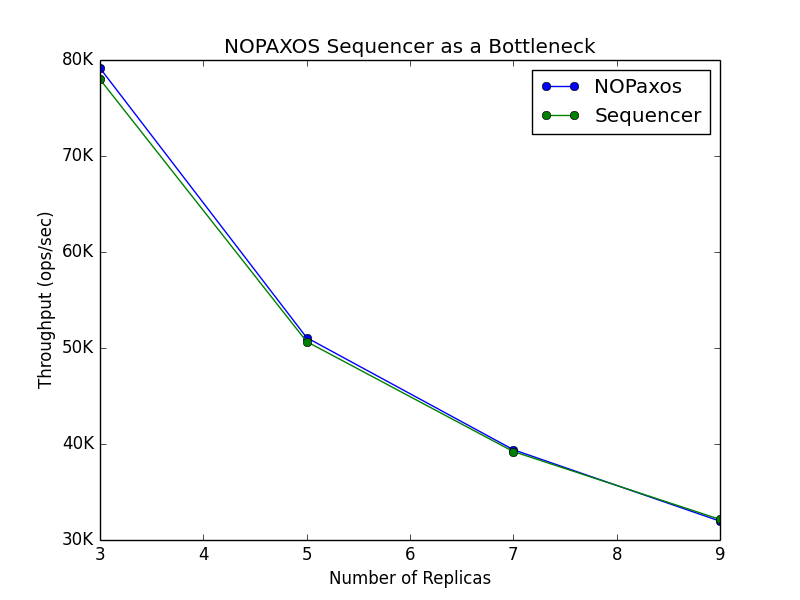
\includegraphics[scale=0.5]{figures/final_SeqBottleneck.png}
\caption{Effects of sequencer on NOPaxos throughput, showing maximum throughput of system and sequencer with increasing number of replicas}
\end{figure}

A graph of the throughput of NOPaxos with an increasing number of replicas, both at the sequencer node and for the overall system, is shown in Figure 6. We can see that the throughput of the sequencer dictates the throughput of NOPaxos as a whole closely follows that of the sequencer. We think that any slight difference is the result of the way we took our measurements. This supports our hypothesis that the throughput of the sequencer does, in fact, dictate the throughput of the entire system. 

The sequencer is written in C++ using raw sockets, and so is not easily optimized. We experimented with increasing the sequencer's compute power to see if this improved performance, but we saw no changes, confirming that I/O is the bottleneck. Although future work may improve upon the sequencer and thus improve NOPaxos performance as a whole on cloud platforms, we currently see few, if any, opportunities for optimization at the sequencer. As discussed in \ref{related}, many other consensus protocols that reduce performance overhead either make assumptions about the network or the nature of client requests (i.e. commutativity), suggesting that achieving comparable performance to unreplicated without any assumptions is a fundamentally difficult problem. Thus improvement to the sequencer at this point would take significant investigation and innovation. 
\section{Limitations}

As this paper presents work that is not a true reproduction project, but rather is an evaluation of an existing system in a new context, we detail the limitations both of our reproduction of the original NOPaxos paper's results and of NOPaxos as a cloud platform consensus protocol.

\subsection{Reproduction}

Because of the platform on which we selected to evaluate NOPaxos, our results did not confirm those of the original NOPaxos paper; this is as expected. However, there is value in attempting to reproduce precisely the results of any experiment, and we therefore encourage those with dedicated hardware to attempt a focused reproduction project to confirm the results of the original NOPaxos paper. 

\subsection{Inability to Scale}

We have demonstrated that on a cloud platform, while NOPaxos does achieve better performance than its peer consensus protocols, it can only do so at a small scale (between 3-5 replicas and 60K-80K ops/second) because of the necessary modifications to the sequencer. While this may make it a good choice for some systems, systems that require the ability to scale to higher levels of throughput and replication should not use NOPaxos. 

\section{Future Work}

Due to time constraints, we were unable to modify Speculative Paxos to run on a cloud platform and thus were unable to reproduce this comparison from the original NOPaxos paper. We leave it to future work to conduct such an experiment and gather more data on the applicability of network-reliant consensus protocols on cloud platforms. 

Additionally, we were able to experiment only marginally with varying the maximum batch size for the closest competitor of NOPaxos in this paper (Paxos with Batching), choosing ultimately to use the same maximum batch size as was used in the original NOPaxos paper. Our initial experiments showed that increasing or decreasing this maximum batch size noticeably changed the performance of Paxos with Batching with regards to NOPaxos. Although exploring the trade-offs of different batch sizes is beyond the scope of this paper, we encourage future investigations in this area.  

An area that we did not explore in this paper was the performance of NOPaxos and other consensus protocols across different cloud platforms. In particular, there are some (more expensive, less popular) cloud platforms that do allow multicast, the software implementation of which led to a bottleneck in our experiments. A very worthwhile future project would be investigating whether on such a platform, the results of the original paper could be more closely replicated, or if other currently obscured bottlenecks or issues would arise. 

We also mentioned briefly our decision to put all cloud compute nodes in the same geographic location for testing purposes, as doing otherwise severely impacted the throughput and latency it was possible to achieve, and we wanted to test at levels comparable to those in the original paper. However, the ability to provide georeplication is a significant advantage of cloud platforms. It remains an open question whether the latency improvements NOPaxos is able to achieve when nodes are in the same location are still significant (and reproducible) when nodes are distributed across different locations, or if such microsecond-level latencies become undetectable in the presence of greater delays.

Finally, as previously mentioned, we have left further optimization of the sequencer (the current bottleneck of NOPaxos on a cloud platform), to future work, as such improvements require innovation and investment beyond the scope of this paper. 

\section{conclusion}

In this paper, we evaluated the NOPaxos consensus protocol, a protocol that was shown to outperform its peers on dedicated hardware, on a cloud platform. This required modifying a key piece of the protocol, ordered unreliable multicast (OUM), to run in software at the NOPaxos sequencer without multicast rather than in hardware in the network. The results of our experiments showed that while NOPaxos on a cloud platform still achieves better latency than its peers at lower throughput and replication levels, it is unable to scale to the degree that it was able to on dedicated hardware. We also showed that the bottleneck impacting NOPaxos scalability lay at the sequencer, most likely a result of the modifications that pushed the multicast functionality into the sequencer software. We have identified both the limitations of our experiments and areas for future work in this field, and we hope to see more innovation and investigation surrounding the performance of consensus protocols on cloud platforms in the future.  

\section{Acknowledgements}

We would like to thank the authors of the original NOPaxos paper for their helpful suggestions, responsiveness, and willingness to collaborate with us on this project. We would also like to thank the CS 244 instructors and TAs, Nick McKeown, Keith Winstein, Saachi Jain, and Emre Orbay, for their guidance and support.



\bibliographystyle{ACM-Reference-Format}
\bibliography{reference}

\end{document}